\chapter{Language-Driven Development}
\label{lddchapter}

This chapter provides an introduction to Language-Driven
Development. It outlines current problems facing software and
systems developers today, and explains how an integrated
architecture of semantically rich, evolvable languages can provide
huge productivity benefits to industry.

Language-driven development is fundamentally based on the ability
to rapidly design new languages and tools in a unified and
interoperable manner. We argue that existing technologies do not
provide this capability, but a language engineering approach based
on {\em metamodelling} can. The detailed study of metamodelling
and how it can realise the Language-Driven Development vision will
form the focus for the remainder of this book.
%Tony's suggested section on benefits


% = = = = = = = = = = = = = = = = = = = = = = = = = = = = = = = = = = = = = = =


\section{Challenges Facing Developers Today} \label{challenges}

When discussing software and systems engineering, it is only a
matter of time before the topic of managing complexity arises. The
desire to manage complexity was the driving force behind the
emergence of the aforementioned disciplines, and despite many
valiant attempts to master it, the problem is still with us today.
However, we believe that the nature of today's systems are quite
different to those developed when those disciplines emerged, and
in turn the developers of today's systems face different
challenges to those in previous decades. In particular, it is no
longer sufficient to manage complexity alone. Instead, we believe
that most of today's development challenges boil down to a
combination of three important factors: complexity, diversity and
change.

\begin{figure}[htb]
\begin{center}
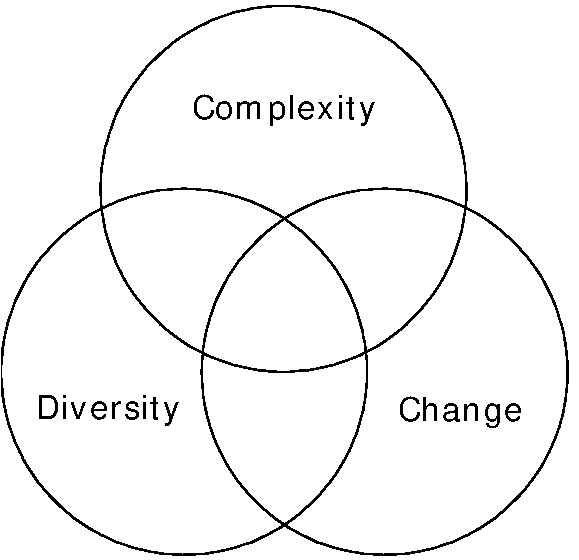
\includegraphics[width=5cm]{LanguageDrivenDevelopment/figures/challenges}
\caption{Challenges Facing Developers Today}
\label{figchallenges}
\end{center}
\end{figure}

The remainder of this section describes each of these challenges in more detail.

\subsection{Coping with Complexity} \label{complexity}

As hardware costs have plummeted and development and manufacture
techniques have improved, the demands for more sophisticated
systems have been relentless. Of course, the more sophisticated
the requirements of a system are, the larger and more complex the
deployed system is likely to be. Increased system complexity
typically brings with it the following problems:
\begin{itemize}
\item longer development times;
\item more complex assembly due to number of components and number of people involved;
\item increased cost and time for testing;
\item increased maintenance costs.
\end{itemize}

Overall, this results in an increased time to market for any
system, and increased development and maintenance costs in order
for there to be any confidence that the quality of the system is
not compromised.

For software systems, as well as the problems outlined above which
relate to the fundamental increase in lines of code, there is an
additional qualitative difference to the systems being developed
today compared to those of decades past. Modern systems are
increasingly distributed in nature, as demonstrated by the
ubiquity of enterprise applications. This adds another dimension
to software complexity, and brings added challenges of
communication and security to those listed above.

Since the challenge of managing complexity is the main topic of
many software and systems engineering books (such as
\cite{sommerville,boochoo,jacobsonoo}, it will not be discussed in
further detail here. Potential solutions to the complexity
challenge are described in section \ref{abstraction}.

\subsection{The Challenge of Diversity} \label{diversity}

The challenge of diversity reflects how developers have to manage
in a non-homogenous environment. Life would be much easier if
there was only one programming language and one deployment
platform, but of course this is not the case, and for very good
reasons. Diversity is not really a single challenge, but a
category of challenges, outlined below. Section \ref{integration}
describes how diversity as a whole can be managed.

\subsubsection*{Diverse Domains}
The requirements of large systems often relate to a variety of
domains that need to be reconciled by different stakeholders.
These requirements may range far and wide, including functional,
safety, security and performance considerations. Each domain often
has its own specialist approach for dealing with appropriate
requirements, but their specialist nature inevitably precludes
them from being applied in other domains.

\subsubsection*{Diverse Customer Requirements}
The 'one size fits all' approach to software and systems is
increasingly inappropriate in today's market. Vendors who offer
products that can be tailored to the specific needs of a customer
have a strong commercial advantage, but developing products that
are truly customisable such that they can meet the demands of a
broad customer base is a far from trivial matter. Despite the fact
that two products being offered to different customers may share
significant functionality, large rewrites and redesign are often
required because the functional components of a system are too
tightly coupled to allow large scale reuse. In addition, many
systems are designed at too lower a level of abstraction to yield
optimum flexibility.

\subsubsection*{Diverse Implementation Technologies}
Systems are often deployed across a number of different
implementation technologies which need to be integrated, or need
to be deployed for a number of separate implementation
technologies. These implementation technologies each have their
own requirements and languages. However, the separation between
the core functionality and the requirements of the deployment
platform is rarely kept clean during the development of the
system. It has been recognised that in order to support
redeployment and integration (or indeed other customisation such
as that described above), systems need to be designed at a high
level of abstraction; thus software and system modelling has
become popular, but these models are rarely complete (this is
described more fully in section \ref{abstraction}). Software
models in particular seldom get beyond the specification of their
behaviour, such that code cannot be completely generated. Even
when code is generated, full testing and validation is usually
required, which consumes a significant chunk of development
effort.

\subsubsection*{Diverse Tools and Artefact Types}
During the development of a system, a large number of artefacts
are created, including requirements specifications, design
documentation, design and analysis models, analysis and simulation
data and of course the code (for software systems). Unfortunately,
these artefacts are often prevented from being truly valuable
assets because:
\begin{itemize}
\item they are often created by different incompatible tools or
using different languages, some of which may no longer be
supported, such that the artefacts become unmaintainable; \item
the forms of artefacts are incompatible, and many are written in
informal languages, such that there is no clear way to integrate
the information they contain; \item artefacts such as design
models are rarely kept in step with changes to the implementation
artefacts such as code, because there is no automatic way to do
so, vastly reducing their value as assets; \item the artefacts
that are kept up to date, such as code, are often tightly coupled
to the integration technology, reducing their value as reusable
assets; \item many artefacts only exist on paper rather than
electronic form, so any maintenance or integration tasks has to be
manually.
\end{itemize}

This may be fine for one-off systems, but systems are rarely built
from scratch - they are often based on existing systems, and as
such would ideally reuse as much as possible from the baseline
system.

\subsection{The Only Constant is Change} \label{change}

Nearly all systems evolve over time. Typical reasons for this are:
\begin{itemize}
\item change in customers requirements or market trends;
\item change in implementation technologies or deployment platforms;
\item support for additional functionality and features;
\item availability of more effective implementation solutions;
\item bug fixes.
\end{itemize}

One can see a parallel between the challenges of change and
diversity described above. The distinction is that diversity is
meant to reflect the potential variations of a system at one point
in time, whereas change is meant to reflect the variation of a
single system over time.

Once again the problem of managing change is intertwined with the
problem of complexity. Traditionally systems have been developed
at too lower level of abstraction, and code is not always the
ideal starting point for managing change.

Ultimately, managing change is costly and timely - system
maintenance is well known to be an expensive activity, and that is
only part of the bigger challenge of managing change. Problems are
compounded when a tool, platform or other technology involved in
the design, development and deployment of the system becomes
obsolete. It can either become even more expensive or in some
cases impossible to continue to maintain a system. It is clear
then that any technique or technology that can aid in managing
change will have a direct beneficial effect on the bottom line and
shorter lead times for delivery. This is the topic of section
\ref{evolvability}.


% = = = = = = = = = = = = = = = = = = = = = = = = = = = = = = = = = = = = = = =


\section{Language-Driven Development - Providing the Solution} \label{lddvision}

\subsection{Languages are the Future} \label{languagesarethefuture}

One of the distinguishing features of being human is our use of
language. Languages are fundamental to the way we communicate with
others and understand the meaning of the world around us.

Languages are also an essential part of systems development
(albeit in a more formalised form than natural languages).
Developers use a surprisingly varied collection of languages. This
includes high-level modelling languages that abstract away from
implementation specific details, to languages that are based on
specific implementation technologies. Many of these are
general-purpose languages, which provide abstractions that are
applicable across a wide variety of domains. In other situations,
they will be domain specific languages that provide a highly
specialised set of domain concepts.

In addition to using languages to design and implement systems,
languages typically support many different capabilities that are
an essential part of the development process. These include:
\begin{itemize}
\item \emph{Execution:} allows the model or program to be tested, run and deployed;
\item \emph{Analysis:} provides information of the properties of models and programs;
\item \emph{Testing:} support for both generating test cases and validating them must be provided;
\item \emph{Visualisation:} many languages have a graphical syntax, and support must be provided for this via the user interface to the language;
\item \emph{Parsing:} if a language has a textual syntax, a means must be provided for reading in expressions written in the language;
\item \emph{Translation:} languages don't exist in isolation. They are typically connected together whether it is done informally or automatically through code generation or compilation;
\item \emph{Integration:} it is often useful to be able to integrate features from one model or program into another, e.g. through the use of configuration management.
\end{itemize}

Languages are the true universal abstractions, and hold the key to
managing the challenges described in section \ref{challenges}.
This section describes how particular facets of languages can help
to solve the individual problems described above, and how they can
combine to from the holistic solution of Language-Driven
Development.

\subsection{Rich Organised Abstraction} \label{abstraction}

Abstraction has long been used as a means to allow humans to cope
with complexity. Abstraction concerns distilling the essential
characteristics of something relative to a particular perspective
of the viewer. The two key ideas here are that some non-essential
details are ignored, and that a particular context needs to be
defined in order for the abstraction to make sense. Often
abstraction involves the `chunking' and organisation of
information in a particular problem domain in order to allow the
viewer to better comprehend the problem, by separating concerns.
It is this information chunking that is the fundamental means for
overcoming the limited human capacity for complexity, and
languages are the means for capturing abstractions.

Organised abstraction is the key tool that formed the basis of the
disciplines of software and systems engineering from the outset
right through to recent trends in model-driven development.
However, there has been a backlash against modelling and concerns
that high-level abstraction doesn't work for complex large scale
systems. This has come from a recognition that current
model-driven technologies have failed to deliver the increased
productivity that was promised. However, we argue that it
abstraction is still a crucial tool - it's just that the wrong
abstractions have been used in the past.

This is partly because there has been a tendency for inappropriate
languages to be used for capturing abstractions - this is covered
in section \ref{multipleLanguages}. More significantly, modelling
languages often use 'high-level' as an excuse to suggest that
their abstractions need not be unambiguous, complete, meaningful
or executable. This simply does not work. Abstraction is a means
of \emph{hiding} detail appropriately from various stakeholders,
but that detail must still be there. Also, if such abstractions
have no meaning or its meaning is ambiguous, then the potential
applications on that abstraction are severely limited -
validation, verification, translation, integration, execution and
simulation rely heavily on semantically precise abstractions.

\subsection{Appropriate Abstraction Through Multiple Languages} \label{multipleLanguages}

Section \ref{diversity} highlighted how diversity lies at the
heart of modern system development. Going a step further, we
suggest that the challenge really boils down to a diversity of
languages:

\begin{itemize}
\item specialists require languages to address the particular facets of the problem that lie within their domain - often within each specialist domain there are numerous languages, with new languages being developed all the time;
\item there are countless implementation languages - some differences are due to the continuing trend of increasing abstraction, some are due to the fact that different paradigms or individual languages are better suited to a particular problem-solution pair than others, and some are simply down to competitive commercial interests;
\item the languages and syntax that capture the artefacts created during the development lifecycle.
\end{itemize}

We propose that rather than trying to subdue this diversity by
forcing everyone to talk (or model) using the same language, we
should embrace it and allow everyone to use whatever language best
suits their needs. In many cases, this may be a general-purpose
modelling or programming language, as these will be widely
supported by tools and techniques, but in some cases more
specialised languages may be more appropriate. An example of this
might be an inventory-based system, where developers consistently
have to express their models in terms of inventory type concepts
such as resources, services and products. By allowing engineers
and domain experts to express themselves in the languages that
they are both most comfortable with and that will give them the
most expressive power, productivity can increase with
corresponding gains for industry.

The argument against this is that by having a single standard
language, there is only one language for developers to learn, so
everyone can communicate more easily, and interoperability between
tools will be much simpler. Whilst this is undoubtedly true, in
order to make a modelling language that suits the needs of
everybody (not just software engineers), it will suffer from the
following problems:
\begin{itemize}
\item it will necessarily be a very large, bloated language;
\item there are often contradictory needs of a language from different domains that cannot be reconciled in a single language;
\item any gain made in widening the applicability of a language to different domains will be at the expense of the richness of the language that makes it so suitable for a particular domain.
\end{itemize}

The compromises that can happen due to conflicting requirements of
a language can be seen clearly in programming languages. These
languages sit uncomfortably between the realms of the computer
hardware and the human developer. As humans, we want readable,
maintainable and reusable code, but ideally we also want to
produce a set of efficient machine instructions to keep the
computer happy. The trend of increasing abstraction that has
resulted in Object-Oriented Programming has resulted in more
usable languages, but at the expense of performance. Thus a single
language is not enough.

\subsection{Integration - Weaving the Rich Tapestry of Languages} \label{integration}

In section \ref{multipleLanguages}, we suggested that large
productivity gains could be achieved by opening up the full
spectrum of languages. However, this vision will not work with
isolated language islands - we need to find a way for all the
models and other artefacts for a system written in these disparate
languages to make sense as a meaningful whole. In order for that
to happen, the languages themselves must be integrated.

Language integration between two languages means that some or all
 of the language constructs of each language are in some way mapped
to corresponding constructs of the other language. Some common
applications of language integration are outlined below:

\subsubsection*{Transformation}
The most publicised application of language integration is that of
transformation, where an artefact in one language is transformed
into an artefact of another. This type of activity is of prime
importance in MDA (see section \ref{mda}), as reflected by
dominance of the concept of transforming Platform Independent
Models (PIMs) to Platform Specific Models (PSMs). Language-Driven
Development goes a step further by enabling high-level models to
be transformed directly into fully compiled executable systems, so
long as the appropriate languages that capture such views of a
system are integrated appropriately. Transformation activities
also include reverse engineering, and generation of any secondary
artefacts such as documentation or even full test beds for
systems.

\subsubsection*{Artefact Integration}
If a system is comprised of a number of subsystems from different
domains, and these different system aspects are described in
different languages, then by integrating the languages, those
aspects can themselves be weaved together to form a unified view
of the system. This is typically used to integrate language
artefacts that are at a similar level of abstraction.

\subsubsection*{Equivalence Verification}
Sometimes it is important to check whether an artefact written in
one language is equivalent to one written in another. For example,
it may be important to check whether an implemented system
conforms to a precise system specification written in a high-level
language. Again if the two languages are integrated appropriately,
then this will be possible.

\subsubsection*{Synchronisation}
Language integration can also enable language artefacts to be
synchronised. For example, whilst in some cases it might be
appropriate to generate code for a system from a high-level model
as a one-shot activity, in many cases it is desirable to keep the
model and code in step. Similarly, if you have a diagramming
language that allows graphical representation of a modelling
languages, it is important to keep the graphical entities in step
with any changes to the model.

\subsection{Evolvability - The Key to Managing Change} \label{evolvability}

Languages evolve in the same way as systems, and the best way to
protect systems against change and obsolescence is to protect the
languages that describe them. They should be flexible and
extensible to cope with changing requirements, and when a new
version of a language is developed, mappings (as described in
section \ref{integration} should be provided to provide full
traceability between versions. In this way, an artefact written in
an earlier version should able to be transformed into the new
version. With some legacy systems, the language is no longer
well-supported. In these cases, the language should be described
and integrated within the Language-Driven Development framework,
such that corresponding artefacts can be transformed into
artefacts in a new more current and appropriate language. In
summary, good language design (see Chapter \ref{langchapter})
together with language integration enables both languages and
systems to evolve in a controlled fashion.

\subsection{Language-Driven Development - The Complete Solution} \label{lddComplete}

This section has described how languages can provide the overall
solution to the challenges described in section \ref{challenges} -
more specifically an integrated framework of semantically rich,
flexible and evolvable languages appropriate to their needs. This
Language-Driven Development framework will:
\begin{itemize}
\item allow the contruction of agile abstractions that are resistant to change;
\item enable those abstractions to be transformed into, integrated with, validated against or synchronised with abstractions written in other languages;
\item support powerful applications (editors, analysis and simulation tools, the aforementioned transformers and integrators) to be written and applied on those abstractions.
\end{itemize}

The right languages enable developers to be significantly more
productive  than using traditional development technologies
because engineers and domain experts can speak in the languages
they understand. Rather than dealing with low level coding issues,
developers can use powerful language abstractions and development
environments that support their development processes. They can
create models that are rich enough to permit analysis and
simulation of system properties before completely generating the
code for the system, and are more reusable and agile. They can
manipulate their models and programs in significantly more
sophisticated ways than they can code. Moreover, provided the
language definitions are flexible, they can adapt their languages
to meet their development needs with relative ease.

Language-Driven Development is the next generation development
paradigm which can provide a step gain in productivity through the
recognition that languages, rather than objects or models, are the
abstractions needed for today's development environment.


% = = = = = = = = = = = = = = = = = = = = = = = = = = = = = = = = = = = = = = =


\section{From Model-Driven to Language-Driven Development} \label{mdd2ldd}

Much of what has been described in this chapter has a lot in
common with  model-driven development approaches such as the OMG's
Model Driven Architecture (MDA). However, there are two prime
motivations for distinguishing Language-Driven Development from
model-driven approaches:
\begin{itemize}
\item the term \emph{model} suggests a focus on high-level abstractions and \emph{modelling} languages, with other artefacts seen as of lesser value. We feel that languages itself are the truly central abstractions, and that modelling languages form an undoubtedly useful yet partial subset of the spectrum of useful languages in system development. Consequently, all language artefacts, not just models, have a crucial role to play in the process;
\item the prominent model-driven approach, MDA, is limited in its scope of application, compared to the full potential of Language-Driven Development (see section \ref{mda}.
\end{itemize}

The remainder of this section examines two key model-driven
technologies from the Object Management Group, UML and MDA, and
assesses their suitability for the basis of Language-Driven
Development.\footnote{Two other key technologies underpinning MDA
are the Meta-Object Facility (MOF) and the
Query/View/Transformations language (QVT). MOF is the
metamodelling language for MDA, and QVT is the mappings language
for MOF - both are described in section \ref{differences}.}

\subsection{The Unified Modelling Language} \label{uml}

The Unified Modelling Language (UML) came out of a desire to
consolidate  all the notations in the various object-oriented
methodologies that had arisen in the eighties and nineties, such
as Schlaer-Mellor \cite{schlaermellor} and OMT \cite{omt}. UML
consists of a number of different notations that allow different
views of a software system to be modelled at different stages of
the development lifecycle. Both static and dynamic aspects of a
system can be captured, and facilities are also provided to enable
model management and limited extensibility. A textual constraint
language (OCL) is included to allow the state space represented by
a model to be further constrained in ways that are too complex to
be captured by the graphical notations alone.

As highlighted earlier, there are certainly advantages of having a
common language such as UML, particularly with regard to
communication. In line with this, UML has been well-received and
is now the \emph{de facto} software modelling language. However,
it has some major shortcomings:

\subsubsection*{Imprecise semantics}

The UML 1.x specification \cite{umlspec} falls some way short of
providing a precise semantics. Whilst its syntax is mostly well
specified, the semantics of those syntactic elements is either
missing or provided informally using English. This has led to a
situation where, as of version 1.3, no tool could claim to be UML
compliant \cite{pumlrfi}. This in turn has inhibited model
interchange between tools, leading back to the situation of vendor
lock-in. In addition, as explained earlier, models written in such
an informally specified language are open to misinterpretation, a
potentially dangerous or expensive problem. Whilst a major
revision of UML will be released soon, draft versions of the UML
2.0 standard do not indicate major improvements with regard to
semantics.

\subsubsection*{Limited scope and flexibility}

UML has been successfully applied across the software development
community, and it is increasingly being applied to non-software
domains such as systems engineering\cite{umlse}, and specialised
software domains such as real time and high integrity systems. The
diverse modelling requirements that this widespread use brings
makes defining what a unified modelling language should be a
considerable problem. Early attempts to enhance UML to support new
requirements adopted a 'mud-packing' approach\cite{kobryn}, which
involved making direct amendments to the monolithic definition of
UML itself. This resulted in a language that became increasingly
large, unwieldy to use, incomprehensible, and difficult to
maintain and test for consistency.

In order to overcome these problems, UML was refactored from a one-size-fits-all modelling language into a family of languages. The foundation of the UML family is a stable core UML metamodel, consisting of minimal modelling concepts that are supported by all family members. Each dialect of UML consists of the UML core
metamodel and one or more extensions to the core known as `profiles'. The profile mechanism is quite straightforward to apply, but is limited as it is based upon constraining existing language constructs rather then modifying or adding new language constructs.

\subsubsection*{Non-executability}

UML is not in itself executable - it was designed to be a
declarative  language. In other words you cannot run a UML model
as defined in the specification, merely define a specification to
which any executable program must conform. This is certainly
useful, but does not (in the general case) allow executable code
to be generated automatically from the model. This was deemed to
be a desirable application of models, so an Action Semantics
extension was provided. Whilst this was a step in the right
direction, like much of UML, the semantics of this extension is
weakly defined.

\vspace{1cm} \noindent These shortcomings are constantly being
addressed by revisions of the language. At the time of writing,
UML 2.0 is due to be released in the near future. This addresses
some of the problems of imprecise semantics, and improves the
profile mechanism of UML 1.4, but it is still limited by the
fundamental flaw of trying to have a one-size-fits-all language.
UML started out as general purpose object-oriented modelling
language, and was good at describing high level object-oriented
software models. But as a consequence of its popularity, attempts
were made to tailor for more and more highly specialised uses for
which it was not originally intended. Developing it as an
extensible language was a major step forward, but the core that
the profiles are built upon is still an object-oriented core,
which does not suit the needs of all languages. We are not
proposing that UML should be scrapped, simply that it used where
it makes sense to use it - and use other languages where the
abstractions provided by UML do not fit.

\subsection{MDA} \label{mda}

The Model Driven Architecture is framework for unifying a number
of technologies based around OMG standards such as UML, MOF, CWM
and CORBA. It is founded on the metamodelling language MOF, which
is used to define other languages such as UML and CWM.

Primarily MDA concerns models and mappings between those models.
The most widely recognised application of MDA is the mapping or
transformation between Platform Independent Models (PIMs) and
Platform Specific Models (PSMs). A key idea is that system models
are constructed that realise all the functional requirements, but
are completely independent of platform, programming language and
other implementation issues (PIMs). Instead of producing code for
a system manually, a model that contains all the constructs and
details needed for the system to operate on the intended
implementation technology (the PSM) is generated from the
appropriate PIM using a mapping. Because the core functionality of
a system is captured in the PIM, if that system needs to be
deployed on to a new platform, a new PSM can be generated simply
by changing the PIM to PSM mapping. Thus faster platform migration
and platform independence are achieved through the large scale
reuse that PIMs provide \cite{mdaexec}.

MDA is an ambitious vision that could change the way software is
developed in the future. However, as with UML, it has some
problems:
\begin{itemize}
\item whilst the MDA vision is grand, the technology for implementing it is very vaguely specified. So weak in fact that any modelling tool which has some simple code generation facility can (and in most cases does) claim to implement MDA. MDA is more useful as a marketing tool than anything else;
\item MDA is too fixed on the notion of \emph{platform}. What constitutes a \emph{platform} is unclear at best - the transition from the most abstract model of a system to the most refined model may include several stages of models, each which could considered Platform Specific when compared to the previous stage, or Platform Independent when compared to the following stage. In any case, PIM to PSM mappings are just one of a whole spectrum of potential applications of Language-Driven Development;
\item MDA is built on a weak inflexible architecture. This will be discussed in the context of metamodelling in section \ref{metaarch}.
\end{itemize}

Language-Driven Development is not just about PIM to PSM mappings
- it is about being able to capture all aspects of the software
and systems development process in a unified way, through the rich
tapestry of languages described in section \ref{lddvision}.

% \subsection{Domain Specific Languages}

% Approaches that aim to facilitate the rapid design of languages
% are not new. Domain specific languages have been around for many
% years, for example \cite{dslrefs}. These provide technologies that
% facilitate the rapid generation of parsers, compilers and
% interpreters for languages that target a specific collection of
% domain abstractions. A problem with many of these approaches is
% that they are relatively low level and bespoke. What is required
% is to raise the level of abstraction at which we tackle
% language-definition, while also maintaining consistency with the
% way that important languages like UML are defined.

% Moreover, we think the focus on domain specific languages (as for
% example proposed by Microsoft's recent Whitehore inititiave) is
% not general enough. In reality, developers require a wide spectrum
% of languages from general-purpose to domain-specific. Indeed, in
% our experience, most domain specific language rely on pre-existing
% general-purpose abstractions if they are to be useful. Thus any
% approach to language-driven development must embrace all language
% types, from general-purpose languages to domain specific languages
% (although even here, we feel that the distinction between
% domain-specific and general-purpose is often very blurred).

% = = = = = = = = = = = = = = = = = = = = = = = = = = = = = = = = = = = = = = =


\section{Language Engineering and Metamodelling}

In order for a development process to be truly adaptable, it is
not simply  a case of enabling it to support a number of
pre-defined languages. If a development process limits itself to
the application of a fixed set of languages, it will still
necessarily limit the range of problems that it can address as
well as the potential solutions it can provide. Instead, a
development process should incorporate the ability to adopt and
construct whatever languages provide the best fit. In other words,
on top of the disciplines of Software and System Engineering,
there needs to be a new discipline for Language Engineering.

Language engineering is required whenever the integrated language
framework does not support the problem-solution pair. For example,
if Language-Driven Development is required on a problem domain
that has its own specialist language or if a new programming
language is developed, then that language must be captured in an
appropriate form to support Language-Driven Development
technologies. However language engineering involves not just the
construction of semantically rich languages for capturing
appropriate abstractions (section \ref{abstraction}). It also
involves the integration of such languages within the language
framework (section \ref{integration}) and the evolution of such
languages (section \ref{evolvability}). Thus language engineering
provides the foundation for all we have described in this chapter.

Language engineering is a more complex activity than software and
system engineering needing specialised skills, however only a
fraction of Language-Driven Development practitioners will be
involved in this activity. For most system developers, it will be
sufficient to know that languages need not be static entities, and
that languages can be customised, extended and created as needed.
Some of these language engineering tasks they may be able to carry
out themselves, and some (particularly the creating of new
languages entirely) will have to be carried out by language
specialists.

In order to be able to engineer languages, we need a language for
capturing, describing and manipulating all aspects of languages in
a unified and semantically rich way. This language is called a
metamodelling language. Metamodels (models of languages) are the
primary means by which language engineering artefacts are
expressed, and are therefore the foundation for Language-Driven
Development. While we have motivated Language-Driven Development
in this chapter, the rest of the book will explore how
metamodelling (the process of creating metamodels) can realise the
Language-Driven Development vision.


% = = = = = = = = = = = = = = = = = = = = = = = = = = = = = = = = = = = = = = =


\section{Conclusion}

This chapter has outlined some of that the key challenges facing
developers today are complexity, diversity and change. It has
proposed that Language-Driven Development can help developers to
manage these challenges by utilising the following tools:

\begin{itemize}
\item abstraction through rich languages helps to manage complexity;
\item integration of multiple appropriate languages help to manage diversity;
\item flexible, evolvable languages help manage change.
\end{itemize}

An outline as to how Language-Driven Development differs from
model-driven development was then given, along with an overview of
existing model-driven technologies and their limitations. The
chapter closed with an introduction to the discipline of Language
Engineering, which this book is fundamentally about, and is
described in more detail in the following chapter.

Language-Driven Development provides practitioners with an
integrated framework of rich evolvable languages appropriate to
their needs. Productivity can be increased because engineers and
domain experts can speak in the languages they understand, and
both the problem space and solution space are opened up to their
full extent, and artefacts developed in this way will be more
agile, powerful, reusable and integrated. This approach offers a
paradigm shift beyond object-oriented programming and modelling
that has major implications for industry in terms of cost
reduction and productivity.
